\documentclass[a4paper,twocolumn,11pt,unpublished]{quantumarticle}
\pdfoutput=1
\usepackage[utf8]{inputenc}
\usepackage[english]{babel}
\usepackage[T1]{fontenc}
\usepackage{amsmath,amssymb,amsthm,mathtools}
\usepackage{booktabs}
\usepackage{graphicx}
\usepackage{microtype}
\usepackage{hyperref}
\usepackage[numbers,sort&compress]{natbib}
\usepackage{tikz}
\usepackage{xcolor}
\usetikzlibrary{arrows.meta,positioning,fit,shapes.geometric}

\newtheorem{proposition}{Proposition}
\newtheorem{corollary}[proposition]{Corollary}
\newcommand{\bits}{\{0,1\}}
\newcommand{\E}{\mathbb{E}}
\newcommand{\Ftwo}{\mathbb{F}_2}
\newcommand{\mmd}{\operatorname{MMD}}
\newcommand{\TVD}{\operatorname{TVD}}
\newcommand{\supp}{\operatorname{supp}}
\newcommand{\campaign}{\textsc{Quantum-Campaign-v1}}
\definecolor{draftblue}{HTML}{0072B2}
\definecolor{draftorange}{HTML}{E69F00}
\definecolor{draftpurple}{HTML}{CC79A7}
\definecolor{draftgray}{HTML}{666666}

\title{Conditional Generation with Classically Trainable IQP Circuits}
\author{Anonymous author(s)}
\affiliation{Internal research draft; author metadata withheld pending a submission decision}

\begin{document}
\maketitle

\begin{abstract}
Conditional generation with a single compiled quantum circuit separates three
questions that are often conflated: how the full output distribution responds
to a condition, which training observables can be estimated classically, and
whether the final circuit can be sampled classically.  We study a fixed
$H^{\otimes n}D_\theta H^{\otimes n}$ IQP circuit whose condition enters only
through a frozen affine $R_Y$ product input.  Specializing
established circuit-Fourier theory, every output probability lies in a finite
multivariate signed-sum support.  Refining the known IQP active-generator
expansion for real product inputs, Pauli-$Z$ responses retain only a filtered
binary span and hence can have a smaller condition spectrum.  The same product
reference gives unbiased estimators for selected Pauli moments, an
independent-copy Conditional MMD objective, and phase gradients, with explicit
second-moment and resource bounds.  Here ``classically trainable'' refers only
to access to those quantities; it does not imply efficient output
probabilities, classical sampling, optimizer convergence, or a favorable
landscape.  An adversarial primary-source audit found the probability theorem
to be a direct specialization and the observable formula to be a short
synthesis of prior results.  The first binding novelty gate therefore failed.
Under a frozen 400-run protocol, this decision blocked the planned 16-qubit
PennyLane-Ising feasibility, tuning, primary, spectral, and ancilla branches;
zero full training runs were reserved or executed.  We report the complete
derivations, executable checks, frozen benchmark, immutable kill tree, and
stopped-work artifacts as a mechanism-and-boundary record.  The result is an
internally complete failure-path draft, not a submission-ready novelty claim.
\end{abstract}

\begin{center}
\fbox{\parbox{0.94\columnwidth}{\small\textbf{Draft status (10 August 2026).}
The internal correctness audit passes and the theorem-novelty gate fails.
No Ising model training was released. Independent quantum-information review
and real author metadata are absent. This manuscript must not be submitted in
its present form.}}
\end{center}

\section{Introduction}

Conditional generation asks one model to represent a family of probability
laws $q_\theta(x\mid c)$ selected by an external condition $c$.  In a quantum
circuit Born machine, the most restrictive deployment version of this task is
to keep one compiled gate sequence and one phase vector at every condition.
Only the prepared input may change.  This constraint is operationally sharper
than sharing a parameterization whose effective gate angles are recomputed for
each $c$, and much sharper than storing a separate circuit for every
condition.

Input encodings already determine the accessible Fourier spectrum of a
parameterized quantum model.  Pauli rotation encodings give finite
trigonometric response spaces, and affine or multidimensional encodings map
their base frequencies to signed sums of encoding weights
\cite{gilVidalInputRedundancy2020,schuldEffectDataEncoding2021,
casasMultidimensionalFourier2023}.  This observation constrains each output
probability, but by itself supplies no efficient probability evaluator.
Conversely, probabilistic simulation can estimate selected observables without
strongly simulating the output law \cite{nestSimulatingQuantumComputers2011}.
Recent IQP work makes this distinction concrete through active-generator
Pauli estimators, automatic differentiation, and MMD objectives
\cite{recio-armengolIQPoptFastOptimization2025,
recio-armengolTrainClassicalDeploy2026}.

The technical question in this paper is therefore a three-way boundary.  We
ask how a fixed circuit responds when $c$ changes an affine product input,
which smaller part of that response is visible to classically estimable Pauli
observables, and which conclusions remain unavailable about final output
sampling.  The mechanism is shown in Fig.~\ref{fig:mechanism}.  Its input is
$\bigotimes_iR_Y(b_i+w_i^\mathsf{T}c)|0\rangle$; all generators, their order,
and $\theta$ remain byte-identical across conditions.

\begin{figure*}[t]
\centering
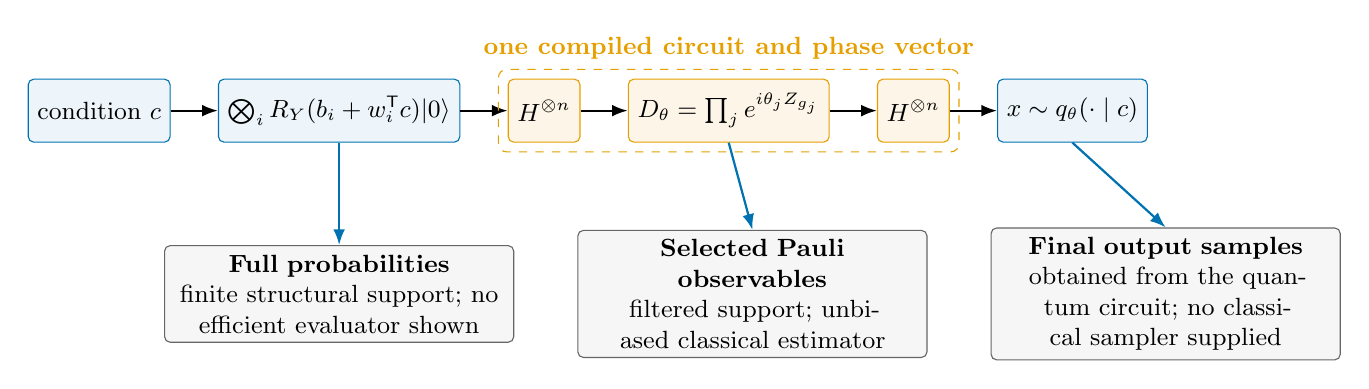
\begin{tikzpicture}[
  node distance=5mm and 6mm,
  box/.style={draw,rounded corners=2pt,minimum height=8mm,align=center,
    font=\small,fill=white},
  qbox/.style={box,draw=draftblue,fill=draftblue!7},
  fixed/.style={box,draw=draftorange,fill=draftorange!9},
  result/.style={box,draw=draftgray,fill=draftgray!6,text width=4.2cm},
  arrow/.style={-{Latex[length=2mm]},thick}
]
\node[qbox] (c) {condition $c$};
\node[qbox,right=of c] (enc) {$\bigotimes_iR_Y(b_i+w_i^\mathsf{T}c)|0\rangle$};
\node[fixed,right=of enc] (h1) {$H^{\otimes n}$};
\node[fixed,right=of h1] (d) {$D_\theta=\prod_j e^{i\theta_jZ_{g_j}}$};
\node[fixed,right=of d] (h2) {$H^{\otimes n}$};
\node[qbox,right=of h2] (out) {$x\sim q_\theta(\cdot\mid c)$};
\draw[arrow] (c)--(enc);
\draw[arrow] (enc)--(h1);
\draw[arrow] (h1)--(d);
\draw[arrow] (d)--(h2);
\draw[arrow] (h2)--(out);
\node[draw=draftorange,dashed,rounded corners=3pt,fit=(h1)(d)(h2),
  label={[font=\small\bfseries,text=draftorange]above:one compiled circuit and phase vector}] {};

\node[result,below=13mm of enc] (p) {\textbf{Full probabilities}\\finite structural support; no efficient evaluator shown};
\node[result,right=8mm of p] (o) {\textbf{Selected Pauli observables}\\filtered support; unbiased classical estimator};
\node[result,right=8mm of o] (s) {\textbf{Final output samples}\\obtained from the quantum circuit; no classical sampler supplied};
\draw[arrow,draftblue] (enc.south) -- (p.north);
\draw[arrow,draftblue] (d.south) -- (o.north);
\draw[arrow,draftblue] (out.south) -- (s.north);
\end{tikzpicture}
\caption{Fixed-circuit conditional generation and the three distinct objects
studied in this paper. Only the product-state input changes with $c$; the
compiled IQP gates and learned phases do not. A structural theorem for full
probabilities is not an efficient probability or sampling algorithm.}
\label{fig:mechanism}
\end{figure*}

Our analysis packages four finite-resource consequences.  First, every output
probability has support contained in a common multivariate signed-sum set.
Second, conjugating a Pauli observable through the IQP block selects
anticommuting generators; grouping their $\Ftwo$ span and using
$\langle Y\rangle=0$ on a real $R_Y$ product input yields a sharper observable
support.  Third, the same representation gives bandwidth, derivative, and
fixed-width non-density statements.  Fourth, the product reference preserves
unbiased selected-moment, Conditional MMD, and phase-gradient estimation.
These are useful specializations and diagnostics, not claims of a new general
Fourier or IQP-estimation framework.

The study was deliberately gated before empirical scale-up.  A written
novelty dossier compared every candidate theorem with primary sources,
attempted counterexamples, and executable small-system checks.  Although the
internal algebra survived, no central result cleared the preregistered
requirement of being more than a direct corollary or short synthesis.  The
binding gate consequently stopped a frozen 16-qubit PennyLane-Ising campaign
before feasibility or model training.  This adverse decision is the primary
campaign result.  It prevents preparatory exact targets, calibration, or older
Gaussian experiments from being repurposed as evidence for an unexecuted
Ising claim.

The contributions that remain supportable are:
\begin{enumerate}
\item an exact deployment contract for affine product-input conditioning of a
fixed IQP circuit, together with a careful separation of probability response,
observable estimation, and sampling;
\item a self-contained specialization of the known full response spectrum and
an observable-specific active-span/real-input filter, with bandwidth,
smoothness, and fixed-resource limitations;
\item explicit finite-variance estimators and operation counts for selected
Pauli moments, sampled Conditional MMD, and phase gradients; and
\item an executable, immutable campaign protocol whose failed theorem gate
provably blocks all 400 allocated full-training runs rather than silently
recycling them.
\end{enumerate}

\section{Related work}

\paragraph{Encoding spectra and expressivity.}
Gil Vidal and Theis characterize Pauli-encoding responses as multiaffine
trigonometric functions and show how repeated affine encodings create signed
frequency sums \cite{gilVidalInputRedundancy2020}.  Schuld, Sweke, and Meyer
derive accessible frequencies from encoding-Hamiltonian eigenvalue
differences and treat multivariate inputs explicitly
\cite{schuldEffectDataEncoding2021}.  Casas and Cervera-Lierta study degrees
of freedom and limitations in multidimensional Fourier series realized by
quantum circuits \cite{casasMultidimensionalFourier2023}.  Our
full-probability statement takes a measurement projector as the observable and
specializes those results to one affine $R_Y$ input per qubit.  It is not a
priority claim.

\paragraph{IQP simulation boundaries.}
Commuting and IQP circuits have sharply different notions of classical
simulation.  Selected quantities can admit probabilistic estimators even when
strong output-probability evaluation is unavailable
\cite{nestSimulatingQuantumComputers2011,
niCommutingQuantumCircuits2012}.  Sampling-hardness results instead depend on
specific circuit families and complexity conjectures
\cite{bremnerClassicalSimulation2011,bremnerAverageCase2016}.  We use no
hardness assumption and make no advantage claim.  Efficient access to the
training observables is kept logically separate from the final act of drawing
an IQP output sample.

\paragraph{Observable-trained IQP models.}
IQPopt develops scalable classical optimization of IQP Pauli objectives and
automatic differentiation \cite{recio-armengolIQPoptFastOptimization2025}.
Recio-Armengol, Ahmed, and Bowles give the active anticommuting-generator
expansion, unbiased Pauli and MMD estimators, and a train-classically/deploy-
quantum workflow \cite{recio-armengolTrainClassicalDeploy2026}.  Our narrow
extension lets the efficiently sampled product reference depend on $c$ and
then evaluates their active expansion on a real affine product input.  The
resulting $Y$ filter and condition-frequency map are convenient diagnostics;
the novelty audit classifies them as a short synthesis.

\section{Fixed-circuit conditional model}
\label{sec:model}

Let $g_j\in\Ftwo^n$ be binary generator masks,
$Z_{g_j}=\bigotimes_iZ_i^{(g_j)_i}$, and define
\begin{equation}
 D_\theta=\prod_{j=1}^{m}e^{i\theta_jZ_{g_j}},\qquad
 U_\theta=H^{\otimes n}D_\theta H^{\otimes n}.
 \label{eq:iqp}
\end{equation}
All $g_j$, their order, and $\theta$ are independent of the condition.  For
$c\in\mathbb R^d$, the fixed encoding is
\begin{equation}
 \alpha_i(c)=b_i+w_i^\mathsf{T}c,\qquad
 |\psi(c)\rangle=\bigotimes_{i=1}^{n}R_Y(\alpha_i(c))|0\rangle,
 \label{eq:encoding}
\end{equation}
where $W\in\mathbb R^{n\times d}$ has rows $w_i^\mathsf{T}$.  Neither $W$ nor
$b$ is learned.  The theorem treats them as arbitrary fixed coefficients; the
campaign chooses one map from target-family-only interval calibration and
shares it across all coupling instances.  The conditional output law is
\begin{equation}
 q_\theta(x\mid c)=|\langle x|U_\theta|\psi(c)\rangle|^2.
\end{equation}

The deployment distinction is structural, not terminological.  A fixed-input
model changes Eq.~\eqref{eq:encoding} and keeps every effective IQP phase
fixed.  A condition-modulated-phase baseline keeps 136 shared coefficients but
maps $c$ into effective gate phases, so its compiled numerical phases vary.
A no-condition model receives one input for all labels.  Separate models use
one independent 136-parameter vector per training condition and are capacity
references, not conditional generators.  The implementation compares
serialized deployment signatures to enforce these distinctions.

\section{Finite-resource response structure}
\label{sec:response}

The following statements are included for completeness and diagnostic value.
Proposition~\ref{prop:full-support} is a direct specialization of established
circuit-Fourier results
\cite{gilVidalInputRedundancy2020,schuldEffectDataEncoding2021}; it is not
presented as new.

\begin{proposition}[Full-probability support]
\label{prop:full-support}
For any fixed post-input unitary and any output $x$, there are coefficients
$Q_{x,s}$ such that
\begin{equation}
 q(x\mid c)=\sum_{s\in\{-1,0,1\}^n}Q_{x,s}
 \exp\!\left(i\left[\sum_i s_iw_i\right]^\mathsf{T}c\right).
 \label{eq:full-support}
\end{equation}
Consequently
\begin{align}
 \supp\widehat q_x&\subseteq\Omega_{\mathrm{full}}(W),\notag\\
 \Omega_{\mathrm{full}}(W)
   &:=\left\{\textstyle\sum_i s_iw_i:s_i\in\{-1,0,1\}\right\},
 \label{eq:omega-full}
\end{align}
with at most $3^r$ distinct frequencies when $r$ rows of $W$ are nonzero.
\end{proposition}

The inclusion can be strict: repeated rows collide, special phases cancel
coefficients, and zero rows add no frequency.  Moreover, Eq.~\eqref{eq:full-support}
does not make a coefficient efficiently computable.  The statement is about
the response class, not strong simulation.

For a measured mask $a\in\Ftwo^n$, write
$X_a=\bigotimes_iX_i^{a_i}$ and define the active set and span
\begin{align}
 \mathcal A(a)&=\{j:a\cdot g_j=1\pmod 2\},\notag\\
 \mathcal H_a&=\operatorname{span}_{\Ftwo}
   \{g_j:j\in\mathcal A(a)\}.
\end{align}

\begin{proposition}[Observable active-span filter]
\label{prop:observable}
Let
\begin{equation}
 f_a(c)=\langle\psi(c)|U_\theta^\dagger Z_aU_\theta|\psi(c)\rangle.
\end{equation}
Then
\begin{equation}
 f_a(c)=\sum_{\substack{h\in\mathcal H_a\\h\wedge a=0}}
 \kappa_h(\theta)
 \prod_{i:a_i=1}\cos\alpha_i(c)
 \prod_{i:h_i=1}\sin\alpha_i(c),
 \label{eq:observable-span}
\end{equation}
where $\kappa_h$ is the sum of the active-generator subset coefficients whose
binary XOR equals $h$.  Write $S_{a,h}=\supp(a)\cup\supp(h)$.  Then
\begin{align}
 \supp\widehat f_a
   &\subseteq\bigcup_{\substack{h\in\mathcal H_a\\h\wedge a=0}}
     \Omega_{a,h},\notag\\
 \Omega_{a,h}
   &:=\left\{\textstyle\sum_{i\in S_{a,h}}\sigma_iw_i:
     \sigma_i\in\{-1,+1\}\right\}.
 \label{eq:omega-observable}
\end{align}
\end{proposition}

Only generators anticommuting with $X_a$ survive conjugation through
$D_\theta$.  Expanding them produces $X_aZ_h$; after the first Hadamards this
is $Z_aX_h$.  Any overlap $h\wedge a$ introduces a local $Y$, whose expectation
vanishes on the real $R_Y$ product state.  This derivation refines the known
active-subset expansion \cite{recio-armengolTrainClassicalDeploy2026}; the
adverse audit does not assign it independent theorem-level novelty.

\begin{figure}[t]
\centering
\includegraphics[width=\columnwidth]{figures/response_support.pdf}
\caption{Illustrative scalar supports. The full probability support is a
common structural upper bound; an observable can retain only a filtered
subset. Frequencies and coefficients depend on the encoding and circuit, and
permitted components can still vanish.}
\label{fig:response-support}
\end{figure}

Let $B_k=\sum_i|W_{ik}|$.  Trace-norm differentiation of the product input
gives the following finite-resource consequences.

\begin{corollary}[Bandwidth and fixed-width limitation]
\label{cor:bandwidth}
For any fixed effect $M$ with $\|M\|_\infty\leq1$ and
$F(c)=\operatorname{Tr}[MU\rho(c)U^\dagger]$,
\begin{equation}
 |\partial^\gamma F(c)|\leq\prod_{k=1}^{d}B_k^{\gamma_k}.
 \label{eq:derivative}
\end{equation}
Along direction $v$, the $r$th derivative is at most
$(\sum_i|w_i^\mathsf{T}v|)^r$.  For $f_a$, both sums restrict to the active
observable lightcone.  For fixed $n,W,b$, the resulting probability-valued
maps are not dense in the continuous probability families on any compact set
with nonempty interior.
\end{corollary}

The non-density statement follows because the finite-dimensional span of
Eq.~\eqref{eq:omega-full} is closed: a two-outcome target containing a cosine
at any frequency outside that span has a positive uniform approximation
floor.  It says nothing about a sequence whose width, re-upload depth, or
encoding weights grow.  Likewise Eq.~\eqref{eq:derivative} describes response
regularity, not gradient magnitude or optimization landscapes.

\section{Classical estimation of the training objective}
\label{sec:estimator}

Set $|\chi(c)\rangle=H^{\otimes n}|\psi(c)\rangle
=\sum_z\phi_c(z)|z\rangle$ and $\pi_c(z)=|\phi_c(z)|^2$.  The $R_Y$ input makes
both objects products of local terms, so a reference string can be sampled and
its amplitude evaluated in $O(n)$ operations.  Define
\begin{equation}
 \Phi_\theta(z)=\sum_j\theta_j(-1)^{g_j\cdot z}
\end{equation}
and, with value zero outside the support of $\pi_c$,
\begin{equation}
 R_{a,c,\theta}(z)=
 \frac{\phi_c(z\oplus a)}{\phi_c(z)}
 e^{i[\Phi_\theta(z\oplus a)-\Phi_\theta(z)]}.
 \label{eq:ratio}
\end{equation}

\begin{proposition}[Product-reference estimator]
\label{prop:estimator}
For $z\sim\pi_c$,
\begin{equation}
 \E\operatorname{Re}R_{a,c,\theta}(z)=f_a(c),\qquad
 \E|R_{a,c,\theta}(z)|^2\leq1.
 \label{eq:second-moment}
\end{equation}
Only $j\in\mathcal A(a)$ enter the phase difference.  Since $\pi_c$ is
independent of $\theta$, termwise differentiation is unbiased; each active
gradient component has second moment at most four and every inactive component
is exactly zero for that observable.
\end{proposition}

The estimator is finite-variance but not pointwise bounded: a rare reference
outcome can carry a large amplitude ratio.  The ordinary $S$-sample mean has
RMSE at most $S^{-1/2}$ and admits a Chebyshev guarantee.  A median-of-means
wrapper gives logarithmic failure-probability dependence but is not generally
unbiased.  A Hoeffding bound for the raw ratio would be unjustified.

For the Hamming kernel
$k_\sigma(x,y)=\exp[-d_H(x,y)/(2\sigma^2)]$, a product distribution over
binary masks represents the kernel as a mixture of Pauli characters.  With
$p_\sigma=(1-e^{-1/(2\sigma^2)})/2$ and
$q_\sigma(a)=p_\sigma^{|a|}(1-p_\sigma)^{n-|a|}$,
\begin{equation}
 k_\sigma(x,y)=\sum_{a\in\bits^n}q_\sigma(a)
 (-1)^{a\cdot x}(-1)^{a\cdot y}.
 \label{eq:hamming-character-mixture}
\end{equation}
This is the product mask law used by the IQP MMD estimator
\cite{recio-armengolTrainClassicalDeploy2026}.  A naive
square of one estimated character mean is biased; independent cross-products
or the corresponding U-statistic yield an unbiased squared discrepancy
\cite{grettonKernelTwoSample2012}.  Averaging the three frozen bandwidths
$\sigma\in\{1,2,4\}$ and balancing conditions produces the sampled
Conditional MMD objective.  Because masks, target minibatches, and product-
reference samples are phase independent, autodifferentiating that finite
sample expression gives an unbiased phase-gradient estimator.

\begin{center}
\fbox{\parbox{0.94\columnwidth}{\small\textbf{Operational definition.}
In this paper, \emph{classically trainable} means that the declared polynomial
mixture of Pauli moments, its sampled Conditional MMD loss, and phase gradients
are accessible to a classical estimator with polynomially declared budgets.
It does not mean efficient arbitrary output probabilities, efficient classical
output sampling, guaranteed convergence, nonvanishing gradients, absence of
barren plateaus, or quantum advantage.}}
\end{center}

With local amplitudes cached, one reference sample costs $O(n)$ to draw,
$O(|a|)$ for its flip ratio, and
$O(\sum_{j\in\mathcal A(a)}|g_j|)$ for the active phase.  For $C$ conditions,
$R$ sampled observables, and $S$ shared reference samples per condition, the
direct batched cost is
\begin{equation}
 O\!\left(CS\left[n+\sum_{r=1}^{R}
 \left(|a_r|+\sum_{j\in\mathcal A(a_r)}|g_j|\right)\right]+Cnd\right).
\end{equation}
Writing a dense $m$-component gradient necessarily costs $\Omega(m)$.  These
counts separate qubit number, generator growth, condition count, and condition
dimension; they are not claims about landscape trainability.

\subsection{Synthetic scaling along declared resource axes}

A zero-training-run audit used frozen synthetic parameters to vary qubits,
generators, condition count, and condition dimension on both a bounded-degree
$O(n)$ generator track and a Complete 2-local $O(n^2)$ track.  Its 21 cases
cover $n\in\{4,8\}$, 8--36 generators, $K\in\{1,4,16\}$ conditions, and
$d\in\{1,2,4\}$ condition dimensions, using 256 reference samples in each of
three independent repeats.  Fourteen $n=4$ cases admit exact statevector
references; their worst expectation RMSE was 0.0583 and worst active-coordinate
gradient RMSE was 0.128.  The seven $n=8$ cases use repeated-estimator
consistency instead of an exact reference in this audit; their worst
consecutive-repeat RMSE was 0.0738 for the expectation and 0.130 for active
gradients.  Per-case wall time, process peak RSS, the Python/JAX/device
environment, exact invocation, code revision, and source digests are archived.
Timing and memory are host dependent; deterministic inputs, draws, numerical
summaries, and their digest are separated from them.  These are
estimator error and resource measurements, not evidence about raw gradient
magnitude, optimizer convergence, or landscape trainability.

\section{Frozen Ising campaign and kill tree}
\label{sec:campaign}

The empirical protocol was frozen before model results so that an adverse gate
could not be repaired by changing targets, thresholds, or run allocation.  It
uses the official periodic random-positive $4\times4$ PennyLane-Ising
construction \cite{pennylaneIsingDataset2026,pennylaneIsingGenerator2026}.
For each coupling instance we exactly enumerate all $2^{16}=65{,}536$ strings,
with energy $E(s)=-\tfrac12s^\mathsf{T}Js$ and target
$p_\beta(s)\propto e^{-\beta E(s)}$.  Seed 666 anchors the released generator;
seven additional coupling seeds and aligned data seeds are frozen.

Target-only calibration screened declared intervals using exact adjacent-beta
TVD, normalized entropy, and endpoint concentration.  The widest eligible
interval was $[0.15,0.55]$, with five training points including $\beta=1/3$
and four adjacent held-out midpoints.  This artifact and eight exact target
archives were generated while the theorem audit was open.  They are
preparatory evidence only: the target-calibration gate was never released
because its predecessor failed.

\begin{table*}[t]
\centering
\caption{Frozen, unexecuted Ising mechanism benchmark. Held-out conditions are
inaccessible to calibration, tuning, feature selection, and checkpoint
selection. Full-training-run use is zero because the first gate failed.}
\label{tab:protocol}
\small
\begin{tabular}{lll}
\toprule
Component & Frozen rule & Status \\
\midrule
Targets & $8$ periodic $4\times4$ instances; exact $2^{16}$ truth & Preparatory only \\
Input & One target-family-calibrated affine $R_Y$ map, shared by all instances & Declared \\
Ansatz & Complete 2-local IQP; $16$ qubits, $136$ phases & Declared \\
Controls & Phase-modulated, no-condition, and separate models & Declared \\
Data & $5{,}000$ Training; $2{,}000$ disjoint Validation strings & Not certified \\
Objective & Balanced batches; $2{,}000\times2{,}000$ estimator budget & Not run \\
Primary & $8\times5\times(3+5)=320$ full training runs & Blocked \\
Statistics & Exact held-out TVD; paired hierarchical bootstrap & Blocked \\
Ancillas & $m\in\{3,5\}$ and matched-capacity controls & Cancelled \\
\bottomrule
\end{tabular}
\end{table*}

The run ledger is content addressed.  A run identity includes the campaign
version, stage, coupling and data seeds, condition scope, model family,
phase-feature candidate when applicable, ancilla rung, optimizer seed, and
manifest digest.  A terminal result must additionally record code revision,
environment, exact invocation, timestamps, runtime, peak memory, parameter
accounting, dataset hashes, estimator randomness, checkpoint provenance, raw
metrics, and completion state.  Reservations and results are immutable;
duplicate or undeclared identities are rejected.

\begin{figure*}[t]
\centering
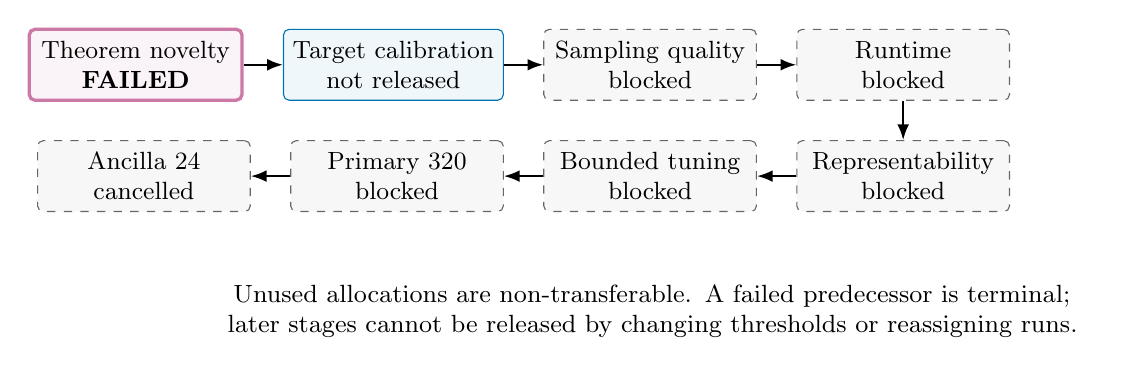
\begin{tikzpicture}[
  node distance=5mm and 5mm,
  gate/.style={draw,rounded corners=2pt,minimum width=2.7cm,minimum height=9mm,
    align=center,font=\small},
  fail/.style={gate,draw=draftpurple,very thick,fill=draftpurple!9},
  blocked/.style={gate,draw=draftgray,dashed,fill=draftgray!5},
  prep/.style={gate,draw=draftblue,fill=draftblue!6},
  arrow/.style={-{Latex[length=2mm]},thick}
]
\node[fail] (nov) {Theorem novelty\\\textbf{FAILED}};
\node[prep,right=of nov] (cal) {Target calibration\\not released};
\node[blocked,right=of cal] (sample) {Sampling quality\\blocked};
\node[blocked,right=of sample] (runtime) {Runtime\\blocked};
\node[blocked,below=of runtime] (repr) {Representability\\blocked};
\node[blocked,left=of repr] (tune) {Bounded tuning\\blocked};
\node[blocked,left=of tune] (primary) {Primary 320\\blocked};
\node[blocked,left=of primary] (anc) {Ancilla 24\\cancelled};
\draw[arrow] (nov)--(cal);
\draw[arrow] (cal)--(sample);
\draw[arrow] (sample)--(runtime);
\draw[arrow] (runtime)--(repr);
\draw[arrow] (repr)--(tune);
\draw[arrow] (tune)--(primary);
\draw[arrow] (primary)--(anc);
\node[below=8mm of tune,font=\small,align=center,text width=11cm]
{Unused allocations are non-transferable. A failed predecessor is terminal;
later stages cannot be released by changing thresholds or reassigning runs.};
\end{tikzpicture}
\caption{Binding campaign kill tree and realized state. Preparatory exact
targets do not bypass a failed predecessor. No feasibility, representability,
tuning, primary, spectrum, or ancilla model run was launched.}
\label{fig:kill-tree}
\end{figure*}

The full allocation is 20 feasibility/representability, 36 tuning, 320
primary, and 24 conditional ancilla runs.  These are independent ceilings, not
a fungible total.  Monotonic gate records ensure that a theorem failure makes
every downstream reservation ineligible.  Tiny exact fixtures exercise the
same transitions, model relations, leakage checks, result schemas, and
statistics without consuming campaign runs.

\section{Evidence and adverse novelty decision}
\label{sec:evidence}

The internal dossier contains exact assumptions, complete proofs, a
primary-source matrix, counterexample attempts, executable checks, and a
claim-evidence registry.  Twenty-one focused theorem tests cover signed-sum
enumeration, frequency collisions, exact small-circuit Fourier support,
active-generator parity, binary spans, the real-input $Y$ filter, joint-XOR
survivors, inactive-phase cancellation, and bandwidth calculations.  These
checks support correctness only; they cannot establish novelty.

\begin{table*}[t]
\centering
\caption{Closest-primary-result audit. ``Delta'' is the strongest accurate
difference found, not a novelty claim. The binding requirement was at least one
correct central theorem that was not a direct corollary or short synthesis.}
\label{tab:novelty}
\small
\begin{tabular}{llll}
\toprule
Candidate & Closest primary result & Residual delta & Verdict \\
\midrule
Probability support & Gil Vidal--Theis; Schuld et al. & Projector packaging & Specialization \\
Bandwidth & Gil Vidal--Theis; Casas et al. & Explicit fixed-$W$ counterfamily & Corollary \\
Observable span/filter & Recio-Armengol et al. & Real-input evaluation & Short synthesis \\
Reference estimator & Van den Nest; IQPopt & Resource-axis accounting & Specialization \\
\bottomrule
\end{tabular}
\end{table*}

The combined active-span formula was not found verbatim, but absence of an
identical displayed equation is not evidence of a central conceptual advance.
Its ingredients and cancellation mechanism are explicit in the closest IQP
work, and the remaining step is a short Pauli-algebra/Fourier synthesis.  The
novelty criterion therefore fails even though the statements survive the
present internal checks.

\begin{table}[t]
\centering
\caption{Full-training-run ledger at the stop decision. Allocated runs remain
unspent and cannot be moved to another pool.}
\label{tab:ledger}
\footnotesize
\begin{tabular}{@{}lrrr@{}}
\toprule
Pool & Cap. & Reserved & Done \\
\midrule
Feasibility/representation & 20 & 0 & 0 \\
Tuning & 36 & 0 & 0 \\
Primary & 320 & 0 & 0 \\
Ancilla & 24 & 0 & 0 \\
\midrule
Total & 400 & 0 & 0 \\
\bottomrule
\end{tabular}
\end{table}

Two complete sampler-development attempts preceded the final novelty verdict.
With 2,000 burn-in sweeps and thinning intervals of 10 or 16, each missed the
frozen per-chain energy-ESS threshold in 2 of 40 Validation cells; all other
exact-reference moment, correlation, and low-weight-character checks passed.
A more conservative 32-thinning attempt was interrupted immediately when the
theorem verdict arrived, after six cells.  These archived attempts neither
pass the sampling gate nor consume full training runs.  No model saw their
samples.

One older 19-qubit Gaussian Hamming-profile study explains why the structured
untwirled Ising benchmark was proposed.  Across ten optimizer seeds in its
archived protocol, the shared angle-conditioned model had mean-condition
profile TVD $0.096$ and Bitstring TVD $0.314$, compared with $0.365$ and
$0.482$ for no condition.  The gap between profile and Bitstring fidelity
motivated exact untwirled evaluation on a non-shell target.  It is historical
motivation, not evidence for any of the blocked Ising claims; the full legacy
audit is confined to the supplement.

\section{Discussion}

The fixed-input deployment contract remains conceptually useful.  It rules out
condition-dependent gate reprogramming and makes the source of conditional
capacity explicit.  The response calculation then separates a common full
probability support from an observable-specific active span, while the product
reference isolates exactly which training quantities remain classically
estimable.  This vocabulary prevents a finite-spectrum expressivity statement
from being mistaken for strong simulation and prevents autodifferentiation
from being mistaken for a landscape guarantee.

The same clarity exposes why the intended theory-led paper cannot proceed.
The full support is a direct instance of general circuit-Fourier theory.  The
IQP refinement is useful bookkeeping but combines ingredients already explicit
in the active-generator literature.  Smoothness, fixed-width non-density, and
the estimator follow by short consequences or specialization.  Running 320
primary fits would at best supply evidence for a mechanism whose proposed
theoretical headline had already failed the campaign's significance rule.
Stopping is therefore not missing experimental work; it is the prescribed
outcome of the experimental design.

No inference can be made about Ising representability, benefit retention,
held-out interpolation, unresolved target spectral mass, or ancilla
marginalization.  Likewise, the analysis does not show conditional
universality, BQP universality, efficient arbitrary probabilities, efficient
classical sampling, optimizer convergence, immunity to barren plateaus,
classical superiority, hard sampling for the finite instances, or quantum
advantage.  The exact 16-qubit targets and calibrated grid are protocol-
development artifacts, not a substitute for the blocked comparison matrix.

A new campaign version could be justified only by a materially different
central result.  Plausible directions include a topology-dependent
approximation lower bound using the active-generator code structure, algebraic
constraints on attainable observable coefficients beyond frequency support,
or a target-spectral excess-risk bound that predicts an independently observed
interpolation boundary.  Any candidate must undergo a new primary-source and
proof audit, followed by independent specialist review, before model training
is released.

\section{Conclusion}

We specified conditional generation with one fixed IQP circuit and an affine
product-state input, then separated the resulting probability response from
the selected observables used for training and from final output sampling.
Established Fourier theory gives the finite full-probability support; the
known IQP active expansion plus the real-input filter gives a sharper Pauli
response; and a product-reference ratio gives finite-variance access to the
declared Pauli, Conditional MMD, and phase-gradient quantities.

The strongest empirical fact in the frozen campaign is that no full training
run occurred.  An internally correct theorem package failed the binding
novelty test, so the immutable protocol blocked every downstream Ising and
ancilla stage.  That stop preserves the distinction between an explanatory
synthesis and a publishable central advance.  The present package is a
reproducible mechanism-and-boundary record; it is not ready for submission to
\emph{Quantum} without a genuinely new result, a new campaign version, real
author metadata, and independent expert review.

\onecolumn
\appendix
\section{Complete analytical details}
\label{app:proofs}

This supplement gives the complete internal derivations behind
Sec.~\ref{sec:response} and Sec.~\ref{sec:estimator}.  They are recorded for
correctness and reproducibility.  As established by the closest-primary-result
audit in Table~\ref{tab:novelty}, the full-probability result is a direct
specialization of circuit-Fourier theory and the observable result is a short
synthesis of the known IQP active-generator expansion with the real-input
filter.  The proofs below are not presented as priority claims.

\subsection{Proof of Proposition~\ref{prop:full-support}}

The density operator of one encoded qubit is
\begin{equation}
 \rho_i(\alpha_i)=R_Y(\alpha_i)|0\rangle\!\langle0|R_Y(\alpha_i)^\dagger
 =\frac12\left(I+\sin\alpha_iX+\cos\alpha_iZ\right).
 \label{eq:local-rho}
\end{equation}
Every matrix entry of Eq.~\eqref{eq:local-rho} is a linear combination of the
three angle frequencies $-1,0,+1$.  Tensoring the local states therefore gives
fixed matrices $A_s$ such that
\begin{equation}
 \rho(c)=\bigotimes_i\rho_i(\alpha_i(c))
 =\sum_{s\in\{-1,0,1\}^n}A_s
 e^{i\sum_i s_i\alpha_i(c)}.
\end{equation}
Substituting $\alpha_i(c)=b_i+w_i^\mathsf{T}c$ absorbs the bias into the
coefficient:
\begin{equation}
 \rho(c)=\sum_s\left(A_se^{i\sum_i s_ib_i}\right)
 e^{i(\sum_i s_iw_i)^\mathsf{T}c}.
\end{equation}
For a fixed unitary $U$ and outcome $x$,
\begin{equation}
 q(x\mid c)=\operatorname{Tr}\!\left[
 U^\dagger|x\rangle\!\langle x|U\rho(c)\right]
\end{equation}
is a fixed linear functional of $\rho(c)$, so it introduces no new frequency.
There are at most three choices per nonzero row of $W$.  Zero rows, coincident
signed sums, and coefficient cancellations only shrink the realized set,
which proves Eqs.~\eqref{eq:full-support}--\eqref{eq:omega-full}.

The proof does not use the IQP structure.  It also does not give an efficient
method for evaluating the trace coefficient $Q_{x,s}$; exact evaluation can
still scale as $2^n$.

\subsection{Proof of Proposition~\ref{prop:observable}}

The final Hadamards map the measured operator to $X_a$.  A diagonal generator
with $a\cdot g_j=0\pmod2$ commutes with $X_a$ and cancels between
$D_\theta^\dagger$ and $D_\theta$.  For an active generator,
\begin{equation}
 e^{-i\theta_jZ_{g_j}}X_ae^{i\theta_jZ_{g_j}}
 =X_ae^{2i\theta_jZ_{g_j}}.
\end{equation}
Since all diagonal generators commute,
\begin{equation}
 D_\theta^\dagger X_aD_\theta
 =X_a\prod_{j\in\mathcal A(a)}
 \left[\cos(2\theta_j)I+i\sin(2\theta_j)Z_{g_j}\right].
 \label{eq:active-product}
\end{equation}
Expanding Eq.~\eqref{eq:active-product} over active subsets $S$ produces the
binary mask $h=\bigoplus_{j\in S}g_j$.  Grouping subsets with equal $h$ gives
\begin{equation}
 \kappa_h(\theta)=
 \sum_{\substack{S\subseteq\mathcal A(a)\\
                  \bigoplus_{j\in S}g_j=h}}
 i^{|S|}
 \prod_{j\in S}\sin(2\theta_j)
 \prod_{j\in\mathcal A(a)\setminus S}\cos(2\theta_j).
 \label{eq:kappa}
\end{equation}
Conjugating $X_aZ_h$ through the first Hadamards yields $Z_aX_h$.  The input
is a product with local moments
\begin{equation}
 \langle X_i\rangle=\sin\alpha_i,\qquad
 \langle Z_i\rangle=\cos\alpha_i,\qquad
 \langle Y_i\rangle=0.
\end{equation}
When $h\wedge a\ne0$, at least one local factor is proportional to $Y$ and
the complete product expectation vanishes.  Otherwise it factors into the
sine/cosine product of Eq.~\eqref{eq:observable-span}.

For completeness, every subset contributing to a surviving $h$ has even
cardinality:
\begin{equation}
 |S|\pmod2=\sum_{j\in S}a\cdot g_j
 =a\cdot\bigoplus_{j\in S}g_j=a\cdot h=0.
\end{equation}
Thus the surviving $i^{|S|}$ and $\kappa_h$ are real.  Expanding each local
sine or cosine into its two exponentials proves
Eq.~\eqref{eq:omega-observable}.

An immediate union lightcone is
\begin{equation}
 L(a)=\supp(a)\cup
 \bigcup_{j\in\mathcal A(a)}\supp(g_j).
\end{equation}
The response is independent of all encoding rows outside $L(a)$, but the
binary-span/$Y$ filter can be strictly tighter than this union.

\subsection{Derivative bounds}

Every derivative of Eq.~\eqref{eq:local-rho} with respect to its angle has
trace norm one.  For positive derivative order it has the form
\begin{equation}
 \frac12[u_r(\alpha_i)X+v_r(\alpha_i)Z],\qquad
 u_r(\alpha_i)^2+v_r(\alpha_i)^2=1,
\end{equation}
whose eigenvalues are $\pm1/2$; at order zero $\rho_i$ itself has trace norm
one.  Apply the requested condition-coordinate derivatives successively to
$\rho(c)=\bigotimes_i\rho_i(\alpha_i(c))$.  The product rule gives an ordered
sum of tensor terms, each of trace norm one.  For coordinate $k$, the absolute
coefficients sum to $B_k=\sum_i|W_{ik}|$, hence
\begin{equation}
 \|\partial^\gamma\rho(c)\|_1
 \leq\prod_kB_k^{\gamma_k}.
\end{equation}
Unitary invariance and H\"older's trace inequality yield
\begin{equation}
 |\partial^\gamma F(c)|
 \leq\|M\|_\infty\|\partial^\gamma\rho(c)\|_1,
\end{equation}
which proves Eq.~\eqref{eq:derivative}.  Replacing each coordinate coefficient
by $w_i^\mathsf{T}v$ proves the directional form.  For an observable response,
Proposition~\ref{prop:observable} removes every qubit outside $L(a)$ before the
same argument is applied.

\subsection{Fixed-width non-density}

Fix $n,W,b$ and a compact condition domain $C\subset\mathbb R^d$ with nonempty
interior.  Let
\begin{equation}
 V_\Omega=\operatorname{span}\{c\mapsto e^{i\omega^\mathsf{T}c}:
 \omega\in\Omega_{\mathrm{full}}(W)\}\subset C(C;\mathbb C).
\end{equation}
This finite-dimensional subspace is closed in the uniform norm.  Choose
$\omega_\star$ with neither sign in the finite support.  Distinct real-vector
exponentials are linearly independent on an open set, so
$g(c)=\cos(\omega_\star^\mathsf{T}c)\notin V_\Omega$ and
\begin{equation}
 \delta=\inf_{v\in V_\Omega}\|g-v\|_\infty>0.
\end{equation}
For $0<\epsilon\leq1/2$, define a valid two-outcome family
\begin{equation}
 p(x_0\mid c)=\tfrac12+\epsilon g(c),\qquad
 p(x_1\mid c)=\tfrac12-\epsilon g(c).
\end{equation}
The constant function lies in $V_\Omega$, whereas Proposition
\ref{prop:full-support} puts every $q(x_0\mid\cdot)$ in $V_\Omega$.
Consequently
\begin{equation}
 \sup_{c\in C}|q(x_0\mid c)-p(x_0\mid c)|\geq\epsilon\delta>0.
\end{equation}
This proves the fixed-resource limitation.  It does not apply to a sequence in
which the support itself grows.

\subsection{Proof of Proposition~\ref{prop:estimator}}

Expanding the Pauli expectation in the diagonal basis gives
\begin{equation}
 f_a(c)=\sum_z\phi_c(z)^*\phi_c(z\oplus a)
 e^{i[\Phi_\theta(z\oplus a)-\Phi_\theta(z)]}.
 \label{eq:expectation-expansion}
\end{equation}
On the support of $\pi_c$, multiplication of Eq.~\eqref{eq:ratio} by
$\pi_c(z)=\phi_c(z)^*\phi_c(z)$ reproduces the summand in
Eq.~\eqref{eq:expectation-expansion}.  Terms with zero denominator already
vanish in the original sum, so the zero convention is harmless.  The quantum
expectation is real, proving unbiasedness of the real part.

The second moment is
\begin{equation}
 \E_{z\sim\pi_c}|R(z)|^2
 =\sum_{z:\phi_c(z)\ne0}|\phi_c(z\oplus a)|^2\leq1.
\end{equation}
For $\chi_j(z)=(-1)^{g_j\cdot z}$,
$\chi_j(z\oplus a)=\chi_j(z)(-1)^{g_j\cdot a}$.  Therefore
\begin{equation}
 \Phi_\theta(z\oplus a)-\Phi_\theta(z)
 =-2\sum_{j\in\mathcal A(a)}\theta_j\chi_j(z).
\end{equation}
The sample law is phase independent and the sum is finite, so differentiation
commutes with expectation.  Explicitly,
\begin{equation}
 \partial_{\theta_j}R=
 \begin{cases}
 -2i\chi_j(z)R,&j\in\mathcal A(a),\\
 0,&j\notin\mathcal A(a).
 \end{cases}
\end{equation}
Multiplying the second moment by four proves the active gradient bound.

\subsection{Unbiased finite-sample Conditional MMD}

For one bit $z\in\bits$ and
$p_\sigma=(1-e^{-1/(2\sigma^2)})/2$,
\begin{equation}
 \E_{A\sim\operatorname{Bern}(p_\sigma)}(-1)^{Az}
 =\begin{cases}1,&z=0,\\e^{-1/(2\sigma^2)},&z=1.\end{cases}
\end{equation}
Independence across bits, with $z=x\oplus y$, gives
Eq.~\eqref{eq:hamming-character-mixture} and the product mask law
$q_\sigma(a)=p_\sigma^{|a|}(1-p_\sigma)^{n-|a|}$.  Thus each mask selects one
Pauli character and averaging masks recovers the Hamming kernel.

Fix one condition, bandwidth, and Fourier mask.  For independent target
characters $t_r=(-1)^{a\cdot x_r}$ and independent real estimator values
$f_s=\operatorname{Re}R_{a,c,\theta}(z_s)$, define
\begin{align}
 \widehat\Delta_{a,c}^{2}={}&
 \frac{1}{N(N-1)}\sum_{r\ne r'}t_rt_{r'}
 +\frac{1}{S(S-1)}\sum_{s\ne s'}f_sf_{s'}\nonumber\\
 &-\frac{2}{NS}\sum_{r,s}t_rf_s.
 \label{eq:u-statistic}
\end{align}
Independence makes the three terms estimate the target square, model square,
and cross-product without self-products, so
\begin{equation}
 \E\widehat\Delta_{a,c}^{2}
 =\left(\langle Z_a\rangle_{p_c}
 -\langle Z_a\rangle_{q_\theta(\cdot\mid c)}\right)^2.
\end{equation}
Averaging Eq.~\eqref{eq:u-statistic} over the declared condition-balanced
minibatch, three bandwidths, and Fourier masks is an unbiased Conditional MMD
estimator.  The stochastic value can be negative.  Clipping it or taking its
square root would alter the estimand.  Since every source of randomness is
phase independent, differentiating this same independent-copy expression is
unbiased.

\section{Counterexample and theorem-check dossier}
\label{app:checks}

The executable theorem checks deliberately target overstatements that a
surface-level derivation can miss.

\begin{enumerate}
\item \textbf{Structural support need not be attained.} For one qubit and a
special IQP phase, an output expectation can be constant even though
$\Omega_{\mathrm{full}}$ permits nonzero frequencies.
\item \textbf{Repeated rows collide.} Three scalar rows equal to one produce
only the seven frequencies $-3,-2,\ldots,3$, not 27 distinct components.
\item \textbf{The union lightcone can be loose.} With $a=100$ and $g=110$,
the active union contains qubit two, but the nontrivial term contains a local
$Y$ and the exact response is independent of its angle.
\item \textbf{Active generators can survive jointly.} For $a=100$,
$g_1=110$, and $g_2=101$, each one-generator term is removed, while their XOR
$011$ is disjoint from $a$ and yields a joint
$\cos\alpha_1\sin\alpha_2\sin\alpha_3$ term.
\item \textbf{Inactive phases cancel exactly.} Varying a generator that
commutes with $X_a$ leaves the exact response and its phase derivative
unchanged.
\item \textbf{The amplitude ratio is not pointwise bounded.} Near a zero local
reference amplitude, a rare sampled ratio can diverge even though its second
moment remains at most one.
\item \textbf{Fixed width misses continuous families.} A cosine at a frequency
outside the finite support gives the explicit uniform approximation floor used
above.
\end{enumerate}

The regression suite enumerates the full multivariate support, detects
collisions, Fourier transforms exact small-circuit probabilities, checks
active parity and $\Ftwo$ spans, verifies the two real-input counterexamples,
compares the complete subset expansion against exact statevectors for one to
four qubits, and validates global and lightcone-restricted bandwidths.  The
estimator tests independently compare sampled expectations and
autodifferentiated gradients with exact circuits.  These are internal
correctness checks, not an external proof review.

\section{Primary-source novelty audit}
\label{app:prior}

The audit searched primary journal and arXiv records using combinations of
``IQP'', ``anticommuting generator'', ``observable support'', ``lightcone'',
``affine input'', ``multidimensional Fourier'', ``product state'', and
``expectation estimator'', then followed citations in the closest papers.  It
was not a systematic review of every thesis, patent, language, or citation
descendant.  That search limitation cannot rescue the claim: the located
sources already establish enough of every candidate result to trigger the
adverse criterion.

Gil Vidal and Theis give the $\{-1,0,1\}^n$ angle spectrum, multiaffine
sine/cosine form, and signed sums from affine weights
\cite{gilVidalInputRedundancy2020}. Schuld, Sweke, and Meyer give the general
eigenvalue-difference Fourier theorem and its multidimensional form
\cite{schuldEffectDataEncoding2021}. Casas and Cervera-Lierta analyze
multidimensional degrees of freedom \cite{casasMultidimensionalFourier2023}.
Van den Nest supplies the general tractable-state/operator probabilistic
estimation framework \cite{nestSimulatingQuantumComputers2011}.  The recent
IQP papers give the active anticommuting expansion, subset/XOR cancellation,
Pauli and MMD estimators, and differentiation argument
\cite{recio-armengolIQPoptFastOptimization2025,
recio-armengolTrainClassicalDeploy2026}.  The residual packaging and filter
are useful, but do not satisfy the frozen central-novelty rule.

\section{Synthetic estimator resource-axis audit}
\label{app:estimator-scaling}

The executable audit at
\texttt{results/quantum-campaign-v1/evidence/estimator-scaling.json} is bound
to the campaign manifest but excluded from every full-training-run pool.  It
uses deterministic synthetic angles, affine input maps, observable masks, and
estimator seeds.  The bounded-degree bank contains one-body generators and
cycle edges; the Complete 2-local bank contains all one- and two-body
generators.  One-axis-at-a-time cases vary $n$, generator count, condition
count $K$, and condition dimension $d$.

Every exact small-system record archives signed bias, maximum absolute bias,
empirical variance, and RMSE for the expectation and phase-gradient estimator.
At $n=8$, where the audit does not claim an exact reference, it instead
archives repeat-to-repeat RMSE and coordinatewise standard deviations.  Each
record also includes runtime, process peak RSS, input size and digest, repeat
seeds, generator/active-generator counts, and the explicit interpretation that
gradient magnitude is not a trainability proxy.  Top-level provenance records
the code revision and dirty-tree state, exact invocation, relevant source
digests, Python/JAX/NumPy versions, operating system, backend, and device kind.
The released 21-case archive
has configuration digest
\texttt{d647f220e3791c4eb678934d25f2ab1557e9396055f3b0e7a4a6ffdd04b28674}
and deterministic numerical-results digest
\texttt{54b5a75c383db7d605efe971d185734c00b2b47adcd0d5438cf6f2a77eeddfb0}.
Wall time and memory are intentionally excluded from the latter digest because
they depend on the execution host.  The audit used zero full training runs.

\section{Frozen manifest and deterministic run plans}
\label{app:manifest}

The production manifest has one canonical JSON digest and exact-key schema.
It freezes the following scientific coordinates:
\begin{itemize}
\item coupling seeds $(666,101,202,303,404,505,606,707)$ and aligned data
seeds $(1666,1101,1202,1303,1404,1505,1606,1707)$;
\item optimizer seeds $(0,1,2,3,4)$;
\item training betas
$(0.15,0.241\overline6,1/3,0.441\overline6,0.55)$ and their four adjacent
midpoints;
\item 16 visible qubits and 136 Complete 2-local generators;
\item bandwidths $(1,2,4)$, 2,000 Fourier operators per bandwidth, and 2,000
product-reference samples per operator and condition;
\item eight MCMC chains, 4,000 declared burn-in sweeps, 32 declared thinning
sweeps, 5,000 Training and 2,000 Validation samples per cell, and all sampler
thresholds;
\item balanced batches of 256, at most 2,000 Adam/cosine updates, Validation-
only checkpoint selection, and nine bounded tuning candidates; and
\item 10,000 paired hierarchical bootstrap replicates with seed 20260810 and
all empirical gate thresholds.
\end{itemize}

The declared full-run identities comprise one runtime feasibility run, six
separate-model representability screens, 36 tuning runs, one exact-objective
diagnostic available only after representability failure, 320 primary runs,
and 24 conditional ancilla runs.  The feasibility/representability pool has a
ceiling of 20; its undeclared remainder is intentionally unspendable.  The
phase tuning slice pairs the three preregistered feature maps one-to-one with
the three declared learning-rate schedules, crossed with two pilot instances
and two optimizer seeds.  A primary or ancilla identity cannot be materialized
until a passed tuning gate contains an immutable evidence-bound decision.

The primary 320 count is
\begin{equation}
 8\text{ instances}\times5\text{ seeds}\times
 (3\text{ shared}+5\text{ separate})=320.
\end{equation}
The ancilla 24 count is
\begin{equation}
 2\text{ instances}\times3\text{ seeds}\times
 2\text{ rungs}\times(1\text{ ancilla}+1\text{ control})=24.
\end{equation}
Unused identities in one budget pool cannot be reserved in another.

\section{Ising reconstruction and preparatory calibration}
\label{app:ising}

The public PennyLane generator uses a periodic NetworkX square grid, no local
fields, legacy NumPy seed 666, directed independent edge draws in $[0,2]$, and
arithmetic symmetrization.  The reconstructed seed-666 coupling matrix has
SHA-256
\begin{center}
\texttt{58cd62927e3be95a827e98efb7282af5a62d2232e15953da6362599017989194}.
\end{center}
Scoring the released 55,000 strings at $T=3$ under this matrix gives mean
energy $-18.7718575999$; exact enumeration gives $-18.7697295208$, a difference
of $-2.20649\times10^{-4}$ exact energy standard deviations.  This joint check
protects the coupling order, sign, factor of one half, bit-to-spin map, and
$\beta=1/T$ convention.

\begin{figure}[t]
\centering
\includegraphics[width=0.88\textwidth]{figures/ising_calibration.pdf}
\caption{Preparatory exact target-only calibration. Left: minimum--maximum
adjacent-target TVD and its median for each candidate interval; blue candidates
passed every exact target rule, and the star marks the widest eligible
interval. Right: five training betas and four adjacent held-out midpoints. The
artifact is reproducible but was never released as a passed campaign gate.}
\label{fig:calibration}
\end{figure}

Figure~\ref{fig:calibration} summarizes the model-free screen.  The selected
interval has minimum adjacent TVD $0.2162$, maximum adjacent TVD $0.3996$,
minimum normalized entropy $0.1874$, and maximum point probability $0.3964$,
meeting the frozen limits $0.015$, $0.40$, $0.18$, and $0.40$.  Its calibration
JSON has SHA-256
\begin{center}
\texttt{8d121e4a519766ff0234e00021815b3bcfd740e9fc9284dbf5b2aa448f29f6ae}.
\end{center}
This matching preparatory artifact cannot pass its gate after a failed
predecessor.

\section{Sampler-development audit}
\label{app:sampler}

The frozen distributional sampler criterion is exact-reference RMSE over the
declared complete bank of one- and two-body parity characters, with threshold
0.08.  The audit also archives plug-in empirical Bitstring TVD over all
$65{,}536$ states, but does not gate on it: at 7,000 retained
Training-plus-Validation strings its unseen-cell mass is dominated by
finite-support undersampling.  The character rule is a disclosed
low-order/Fourier distributional diagnostic, not a claim of certified full-law
TVD.

The zero-field target is invariant under a global spin flip.  The
PennyLane-style single-spin Metropolis kernel was therefore augmented by an
independent global flip of each retained state.  This always-accepted
sampler-only transition preserves the exact law and avoids falsely treating a
trapped ferromagnetic sector as model error.  Every attempt records its chain
count, burn-in, thinning, proposal count, symmetry transition, seeds, hashes,
and exact-reference diagnostics \cite{metropolisEquationState1953}.

\begin{figure}[t]
\centering
\includegraphics[width=0.82\textwidth]{figures/sampler_pilots.pdf}
\caption{Complete sampler-development attempts. Each point is the minimum
energy ESS over the eight Validation chains in one instance/beta cell; orange
points miss the threshold. Both schedules fail 2 of 40 cells, so neither is a
certified campaign dataset.}
\label{fig:sampler-pilots}
\end{figure}

The audit also checks maximum chain-energy deviation, pooled energy error,
magnetization, pair-correlation RMSE, and weight-one/two character RMSE against
the exactly enumerated target.  In the two complete attempts, only the ESS rule
failed.  A declared 4,000-burn-in/32-thinning attempt was then started, but the
novelty verdict arrived after six cells and the process was interrupted with
exit 130.  The partial files and interruption note are retained.  No complete
summary exists, no sampling-quality gate passed, and no model consumed the
data.

\section{Binding statistical rules}
\label{app:statistics}

Had the primary matrix been released, coupling instances—not optimizer seeds
or conditions—would have been the primary scientific replicates.  Each of
10,000 bootstrap draws would first resample eight instances with replacement,
then resample the five matched optimizer seeds within each selected instance,
preserving model and condition pairings.  The frozen seed is 20260810 and the
interval is the 95\% percentile interval.

For a held-out cell, define the benefit retention
\begin{equation}
 r=\frac{\TVD_{\mathrm{no}}-\TVD_{\mathrm{fixed}}}
 {\TVD_{\mathrm{no}}-\TVD_{\mathrm{phase}}}.
\end{equation}
The gate requires median $r\geq0.5$ and a strictly positive lower bootstrap
bound.  Missing methods, nonpositive denominators, or incompatible pairings
fail conservatively.

For each held-out midpoint, the Oracle adjacent-beta lookup evaluates the two
neighboring stored training outputs against the exact held-out target and
keeps the lower TVD.  Fixed input must have a strictly positive paired
improvement interval, win at least 75\% of instance-by-held-out-condition
cells, and worsen no instance's mean.  All three components are binding.  The
ancilla rule similarly requires a preregistered rung to beat both $m=0$ and its
matched-capacity visible control in paired median, 75\% cell wins, and both
instance guardrails; both $m=3$ and $m=5$ would be reported.  No values for any
of these rules exist because their predecessor stages were blocked.

\section{Legacy Gaussian motivation and excluded studies}
\label{app:legacy}

Before the Ising campaign was designed, an archived 19-qubit Complete 2-local
study trained one angle-conditioned model on two permutation-invariant
Gaussian Hamming-weight targets.  Its ten optimizer seeds are the replication
units.  Figure~\ref{fig:legacy} illustrates the profile response; the exact
mean-condition profile and Bitstring TVDs were $0.096$ and $0.314$ for angle
conditioning, $0.365$ and $0.482$ for no condition, and $0.364$ and $0.592$ for
a basis-condition control.  Separate fits were capacity references.  The
remaining Bitstring error exposed nonuniformity within Hamming shells and
motivated the untwirled, structured Ising benchmark.

\begin{figure}[t]
\centering
\includegraphics[width=0.88\textwidth]{../results/summary/weight_fit.pdf}
\caption{Legacy Gaussian motivation, regenerated from its archived ten-seed
study. One shared angle-conditioned checkpoint family changes its Hamming-
weight profile with the input; the no-condition output compromises. This is
not Ising evidence and does not override the failed novelty gate.}
\label{fig:legacy}
\end{figure}

Historical sparse-grid, condition-count, topology, ancilla, and negative
audits remain archived in the repository. A target-specific permutation twirl
can make Bitstring TVD equal profile TVD for a known distribution that is
uniform within Hamming shells, but it changes the output protocol and does not
show that the untwirled circuit learned the symmetry.  Those results are not
part of the present central evidence line and cannot rescue the blocked Ising
campaign.

\section{Reproducibility inventory}
\label{app:reproducibility}

The package provides the following independently inspectable layers:
\begin{enumerate}
\item a strict JSON manifest whose digest binds model, data, estimator,
training, statistical, and budget rules;
\item exact Ising coupling reconstruction, target enumeration, calibration,
and content-addressed target archives;
\item immutable gate records, reservations, result-bundle schemas, and
monotonic stage release;
\item deployment signatures, phase-feature maps, role-tagged datasets,
balanced training helpers, and exact-TV evaluation;
\item hierarchical bootstrap, benefit-retention, Oracle, interpolation, and
ancilla decision functions;
\item theorem-support, estimator-scaling, response-spectrum, campaign, and
manuscript audit tests; and
\item deterministic scripts for evidence figures, report tables, the main
manuscript, and this supplement.
\end{enumerate}

The central regeneration commands are:
\begin{verbatim}
uv sync --group dev
uv run pytest
uv run ruff check src scripts tests
uv run python scripts/prepare_ising_campaign.py --targets-only
uv run python scripts/run_ising_campaign.py --stage primary --dry-run
uv run python scripts/generate_quantum_draft_figures.py
uv run python scripts/run_estimator_scaling.py \
  --output /tmp/iqp-cond-estimator-scaling.json
uv run python scripts/audit_response_spectrum.py \
  --output /tmp/iqp-cond-response-spectrum.json  # blocked, exit 2
uv run python scripts/build_campaign_report.py
(cd paper && latexmk -pdf -interaction=nonstopmode \
  -halt-on-error main.tex)
\end{verbatim}
The target-only command rechecks existing exact archives and releases no gate.
The first theorem gate is already terminally failed.  Running either the full
preparation command or a downstream campaign CLI command returns a blocked
status before dataset generation, reservation, or trainer access.  The
repository does not contain or claim persistent Ising checkpoints.

\section{Adversarial review checklist}
\label{app:review}

Before any future external circulation, an independent quantum-information or
QML expert must review the proofs, closest-prior search, estimator scope, and
significance.  A new positive decision must not edit the existing failed gate;
it requires a new manifest version and evidence chain.  The following items
also remain mandatory:
\begin{itemize}
\item replace anonymous metadata and generic contribution/interest statements;
\item validate every DOI and arXiv version against the final bibliography;
\item rerun the complete suite and clean-environment regeneration;
\item inspect every rendered page for blanks, clipping, unresolved references,
and overfull boxes; and
\item archive independent review responses and allow major objections to
reopen the theorem, claims, experiments, or venue decision.
\end{itemize}


\section*{Data and code availability}
The repository contains the frozen manifest, campaign/ledger implementation,
exact Ising target construction, target-only calibration, failed sampler
attempts, theorem dossier and checks, statistical rules, analysis scripts, and
the complete manuscript sources. Large public-source Ising data are used only
for a reconstruction check; final target truth is generated by exact
enumeration. No trained Ising checkpoints exist because the novelty gate
failed.

\section*{Author contributions and generative-AI use}
The anonymous author(s) designed the study, derived and checked the analysis,
implemented the software, audited the evidence, and wrote the manuscript. This
generic internal statement must be replaced with named CRediT-style
contributions before any submission.
OpenAI Codex assisted with software implementation, literature organization,
test generation, figure and manuscript drafting, and consistency checks. The
human author(s) remain responsible for verifying every proof, citation,
artifact, and statement before external circulation. No AI system is listed as
an author.

\section*{Competing interests}
No competing-interest declaration has been supplied for this anonymous
internal draft. A verified author declaration is required before submission.

\footnotesize
\bibliographystyle{quantum}
\bibliography{references}

\end{document}
